\documentclass[a4paper,11pt]{article}
\input{/home/tof/Documents/Cozy/latex-include/preambule_doc.tex}
\input{/home/tof/Documents/Cozy/latex-include/preambule_commun.tex}
\newcommand{\showprof}{show them}  % comment this line if you don't want to see todo environment
\setlength{\fboxrule}{0.8pt}
\fancyhead[L]{\fbox{\Large{\textbf{KNN 01}}}}
\fancyhead[C]{\textbf{Prédire la variété d'un iris}}
\newdate{madate}{10}{09}{2020}
%\fancyhead[R]{\displaydate{madate}} %\today
%\fancyhead[R]{Seconde - SNT}
\fancyhead[R]{Première - NSI}
%\fancyhead[R]{Terminale - NSI}
\fancyfoot[L]{\vspace{1mm}Christophe Viroulaud}
\AtEndDocument{\label{lastpage}}
\fancyfoot[C]{\textbf{Page \thepage/\pageref{lastpage}}}
\fancyfoot[R]{\includegraphics[width=2cm,align=t]{/home/tof/Documents/Cozy/latex-include/cc.png}}

\begin{document}
%mettre iris.zip sur site
\section{Problématique}
En 1936, le biologiste \emph{Ronald Fisher} a rassemblé les mesures de trois espèces d'iris. Ces informations permettent de distinguer nettement les différences entre ces variétés. Ce travail de collecte et de classification fournit une quantité importante de données mais ne présente aucune analyse. Cependant, il est possible d'utiliser ces données pour pouvoir classifier un iris inconnu.
\begin{center}
    \begin{tabular}{ccc}
        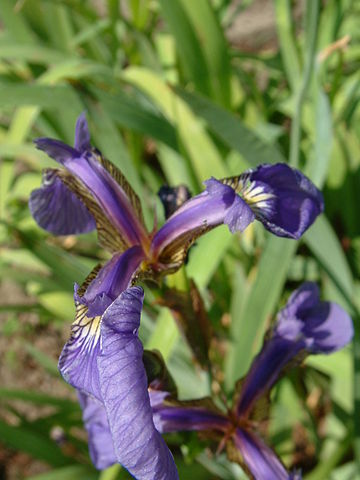
\includegraphics[height=3cm]{ressources/iris-setosa.jpg}&
        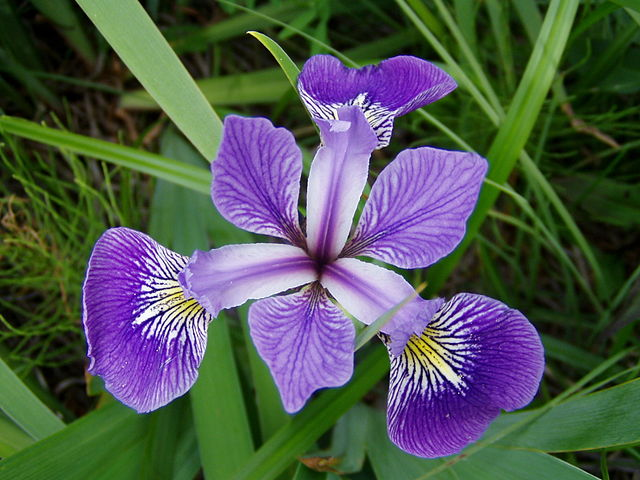
\includegraphics[height=3cm]{ressources/iris-versicolor.jpg}&
        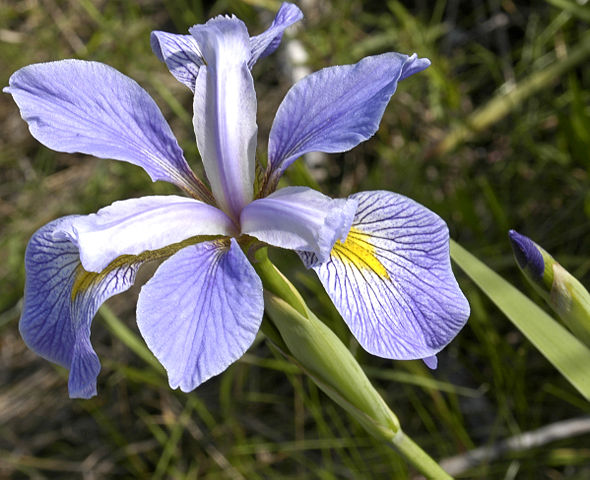
\includegraphics[height=3cm]{ressources/iris-virginica.jpg}\\
        Iris setosa & Iris versicolor & Iris virginica\\
    \end{tabular}
\end{center}
\begin{center}
    \framebox{Comment prédire une information nouvelle à partir de données brutes?}
\end{center}
\section{Utiliser les données}
\subsection{Présentation graphique des informations}
La lecture des données dans un tableau n'est pas très parlante. Une représentation graphique des informations apporte une compréhension plus éclairante.
\begin{center}
\centering
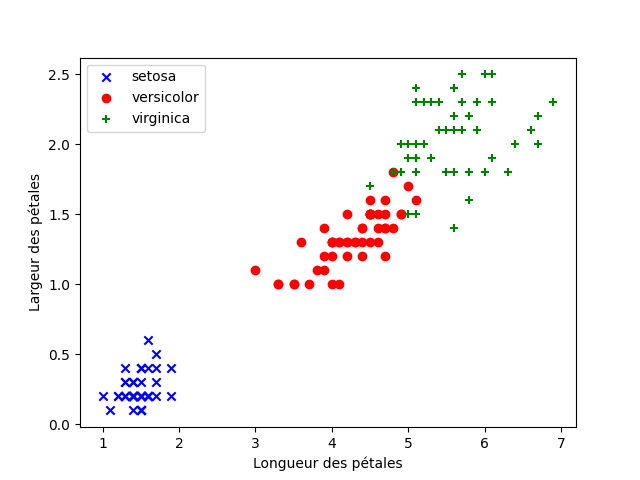
\includegraphics[width=10cm]{ressources/iris-graphe.png}
\captionof{figure}{Variétés d'iris en fonction de leurs mesures }
\label{graphe-iris}
\end{center}
Il apparaît que les mesures d'un iris peuvent permettre de déterminer leur variété.
\subsection{Prédire la variété}
La position d'un iris sur la représentation graphique (figure \ref{graphe-iris}) est caractéristique de sa variété.
\begin{activite}
\begin{enumerate}
    \item Déterminer la variété des iris suivants:
    \begin{tabular}{|*{5}{c|}}
        \hline
        longueur&1&6 &5.1 &2.5 \\
        \hline
        largeur&0.5&2.5& 1.55&0.85 \\
        \hline
    \end{tabular}
    \item Proposer une méthode pour effectuer un choix dans les cas ambigus.
\end{enumerate}
\end{activite}
\section{Algorithme kNN}
\subsection{Présentation}
Pour déterminer la variété d'un iris inconnu, une stratégie consiste à regarder celle d'un nombre \emph{k} de voisins. On attribue alors à la fleur inconnue, la variété la plus présente parmi ses \emph{k} voisins. C'est la méthode des \textbf{k plus proches voisins} (\textbf{k N}earest \textbf{N}eighbors).
\begin{aretenir}[Complément]
L'algorithme \emph{kNN} est une méthode d'apprentissage \emph{supervisé}: l'algorithme reçoit un ensemble de données déjà étiquetées sur lequel il va pouvoir s’entraîner et définir un modèle de prédiction. 
\end{aretenir}
\begin{center}
\centering
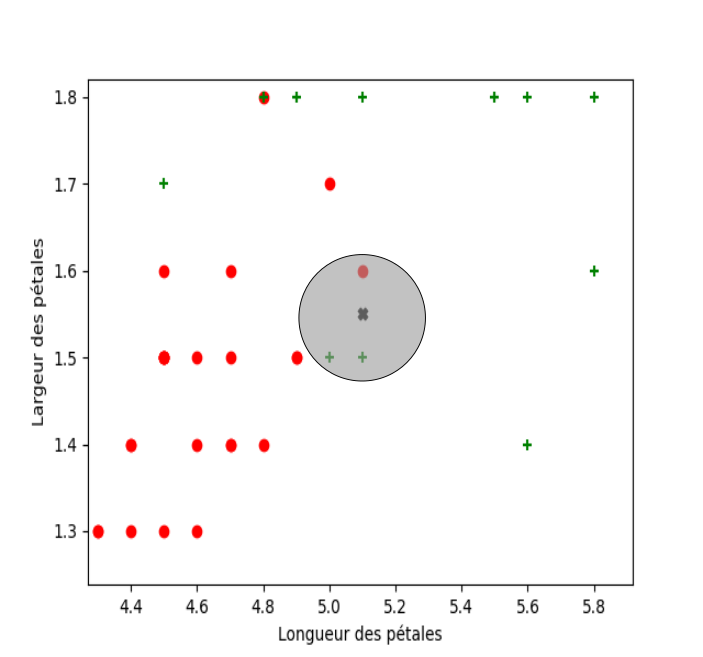
\includegraphics[width=8cm]{ressources/zoom-k3.png}
\captionof{figure}{Détermination de l'iris (5.05, 1.5) pour $k = 3$}
\label{IMG}
\end{center}

\subsection{Construction de l'algorithme}
Une fois la valeur \emph{k} choisie, pour déterminer les plus proches voisins on calcule la distance entre le point \emph{cible} et les autres. Il existe plusieurs manières de calculer une distance. Le plus naturel ici est de prendre la distance \emph{à vol d'oiseau} ou plus formellement la \textbf{distance euclidienne}.
$$d=\sqrt{(x_A-x_B)^2+(y_A-y_B)^2}$$
\begin{activite}
Écrire \emph{en langage naturel}, l'algorithme kNN.

\end{activite}
\subsection{Implémentation}
Les données sont stockées dans un fichier \emph{csv}. Il faut donc d'abord charger ces informations correctement dans le programme avant de pouvoir les utiliser.
\begin{activite}
\begin{enumerate}
    \item Télécharger le dossier compressé \emph{iris.zip} sur le site \url{https://cviroulaud.github.io}
    \item Ouvrir le fichier \emph{data-iris.csv} avec un tableur pour observer les données.
    \item Ouvrir le fichier \emph{iris-eleve.py}.
    \item Compléter la fonction \emph{charger\_donnees} en utilisant les informations du fichier \emph{csv}.
    \item Compléter la fonction \emph{distance} qui calcule le carré de la distance euclidienne entre deux points du plan.
    \item Compléter la fonction \emph{calculer\_distances}.
    \item Compléter enfin la fonction \emph{trouver\_variete}. Le dictionnaire \emph{compteur\_voisins} compte le nombre d'apparitions de chaque variété parmi les \emph{k} voisins.
    \item Tester la fonction avec $k=3$ puis $k=7$, puis pour les autres iris de l'activité 1.
    \item \underline{Pour les plus avancés:} Modifier le code pour tester un ensemble de 10 iris inconnus. De plus chaque iris déterminé sera ajouté au dictionnaire \emph{varietes} afin d'augmenter l'apprentissage de l'algorithme.
\end{enumerate}
\end{activite}

\end{document}